\documentclass[11pt]{mk-polish-lab-report}

\usepackage{lipsum}
\usepackage[normalem]{ulem}
%\usepackage[light, math]{anttor}
\usepackage{array,multirow}

\usepackage{latexsym,amsmath,amssymb,amsthm}
\usepackage{multicol}
\renewcommand{\arraystretch}{1,25}
%\usepackage{amssymb}
\usepackage{breqn}
\usepackage{graphicx}

\let\times\relax% Set equal to \relax so that LaTeX thinks it's not defined
\DeclareMathOperator{\times}{\cdot}
\usepackage{subfig}
\graphicspath{ {plots/} }


%\sisetup{ exponent-product=\cdot}

\university{Politechnika Wrocławska}
\major{Informatyka, inż. I st.}
\tutor{dr hab. Paweł Zieliński}
\coursegroup{czwartek TN, 11:15}

\author{Miriam Jańczak}
\studentnumber{229761}
\title{Obliczenia naukowe}
\topic{Lista 2}


%% Uncomment to change margins size
%\geometry{top=2.5cm,bottom=2cm,left=2.5cm,right=2.5cm}

%% Uncomment to change vspace between items in lists
\setlist[enumerate]{itemsep=0pt}
%\setlist[itemize]{itemsep=0pt}
%\setlist[description]{itemsep=0pt}



\begin{document}

\maketitle

\section{Iloczyn skalarny raz jeszcze}

\subsection{Opis problemu}
Ponowne obliczenie iloczynu skalarnego z zadania~5 z listy~1 dla typów \texttt{Float32} i \texttt{Float64} po wprowadzeniu niewielkich zmian danych w wektorze $x$, tj. obcięciu ostatniej cyfry znaczącej współrzędnych $x_4$ i $x_5$ ($9$ dla $x_4$, $7$ dla $x_5$). W tym celu wykorzystano te same cztery algorytmy co w zadaniu z listy~1. Poniżej przedstawiono zmienione dane wejściowe:
\begin{align}
\tilde{x} = &[2.718281828, -3.141592654, 1.414213562, 0.577215664, 0.301029995] \nonumber \\
y = &[1486.2497, 878366.9879, -22.37492, 4773714.647, 0.000185049] \nonumber
\end{align}

\subsection{Rozwiązanie}
Iloczyn skalarny dla typów \texttt{Float32} i \texttt{Float64} obliczono za pomocą czterech algorytmów z programu z listy~1: 
%\begin{multicols}{2}
\begin{enumerate}[(a)]
\item \textit{w przód},
\item \textit{w tył},  
\item \textit{od największego do najmniejszego},
\item \textit{od najmniejszego do największego}.
\end{enumerate}
%\end{multicols}

\subsection{Wyniki}
Zestawienie wyników iloczynów skalarnych $x\cdot y$ (zadanie~5 z listy~1) oraz $\tilde{x}\cdot y$ przedstawia \Cref{table:1}.

\begin{table}[h]
        \centering
        \footnotesize
\begin{tabular}{c
		|S[
        table-number-alignment = right,
		table-figures-integer  = 2,
		table-figures-decimal = 7
		]
		|S[
        table-number-alignment = right,
		table-figures-integer  = 2,
		table-figures-decimal = 7
		]
		|S[
        table-number-alignment = right,
		table-figures-integer  = 2,
		table-figures-decimal = 16,
		table-figures-exponent=3
		]
		|S[
        table-number-alignment = right,
		table-figures-integer  = 2,
		table-figures-decimal = 16,
		table-figures-exponent=3
		]}
%\toprule
& \multicolumn{2}{c|}{\texttt{Float32}} & \multicolumn{2}{c}{\texttt{Float64}} \\ \hline
{Algorytm}& { $x\cdot y$} & { $\tilde{x}\cdot y$} & { $x\cdot y$} & { $\tilde{x}\cdot y$} \\ \hline
(a) &-0.4999443&-0.4999443&1.0251881368296672e-10&-0.004296342739891585 \\ 
(b) &-0.4543457&-0.4543457&-1.5643308870494366e-10&-0.004296342998713953 \\ 
(c) &-0.5&-0.5&0.0&-0.004296342842280865 \\ 
(d) &-0.5&-0.5&0.0&-0.004296342842280865 \\ 
%\bottomrule
\end{tabular}
\caption{Iloczyny skalarne $x\cdot y$ oraz $\tilde{x}\cdot y$ obliczone w arytmetykach \texttt{Float32} i \texttt{Float64} przy użyciu danych algorytmów.}
\label{table:1}
\end{table}	

\subsection{Wnioski}

\section{Nietypowa granica}

\subsection{Opis problemu}

Porównanie wykresów funkcji
\begin{align}
f(x) = e^x \ln(1 + e^{-x})
\label{eq:zad2}
\end{align}
%$f(x) = e^x \ln(1 + e^{-x})$
(narysowanych w co najmniej dwóch programach do wizualizacji) z jej granicą $\mathop {\lim }\limits_{x \to \infty}$, a następnie wyjaśnienie zaistniałego zjawiska.

\subsection{Rozwiązanie}

Wykresy funkcji \eqref{eq:zad2} wykonano za pomocą biblioteki \emph{Plotly} (używając różnych typów zmiennopozycyjnych) w języku \emph{Julia}, a także za pomocą pakietu matematycznego \emph{Wolfram Alpha}. Granicę $\mathop {\lim }\limits_{x \to \infty}$ funkcji \eqref{eq:zad2} wyliczono za pomocą biblioteki \emph{SymPy} w języku \emph{Julia} oraz w sposób analityczny.  

\subsection{Wyniki}
Poniżej przedstawiono otrzymane wykresy funkcji \eqref{eq:zad2}. 

\begin{figure}[h]
\centering
\subfloat[\texttt{Float16}\label{fig:zad2-fl16}]{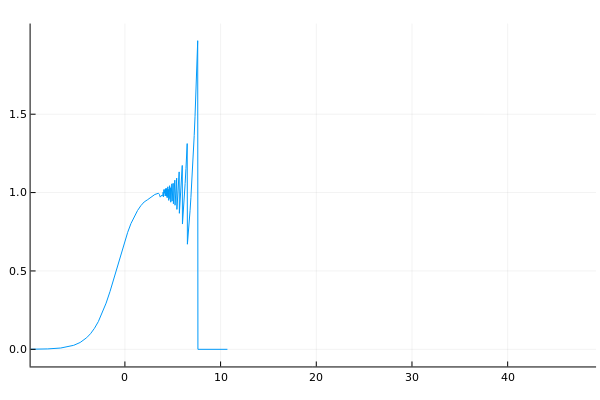
\includegraphics[width=0.5\textwidth]{zad23}}\hfill
\subfloat[\texttt{Float32}\label{fig:zad2-fl32}] {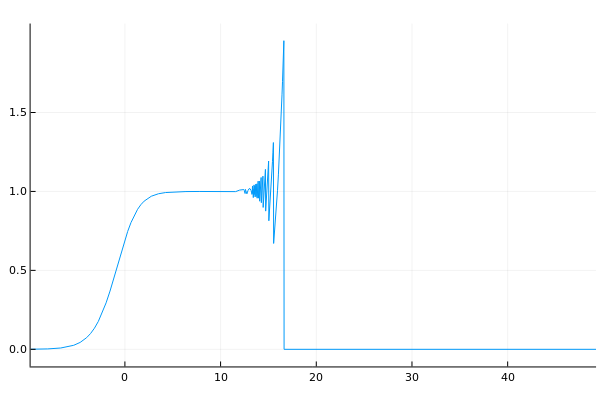
\includegraphics[width=0.5\textwidth]{zad22}}\hfill
\subfloat[\texttt{Float64}\label{fig:zad2-fl64}]{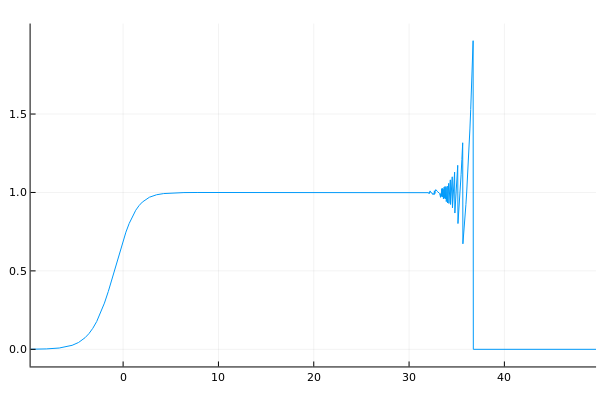
\includegraphics[width=0.5\textwidth]{zad21}}\hfill
\caption{Wykresy wykonane za pomocą biblioteki \emph{Plotly}} \label{fig:zad2-plotly}
\end{figure}

\begin{figure}[h]
\centering
\subfloat[mniejszy zakres \label{fig:zad2-wa1}]{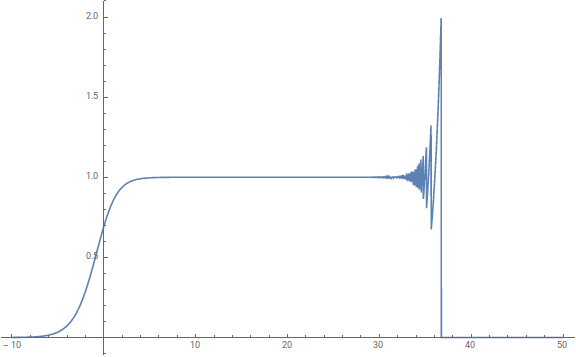
\includegraphics[width=0.49\textwidth]{wa1}}\hfill
\subfloat[większy zakres \label{fig:zad2-wa2}] {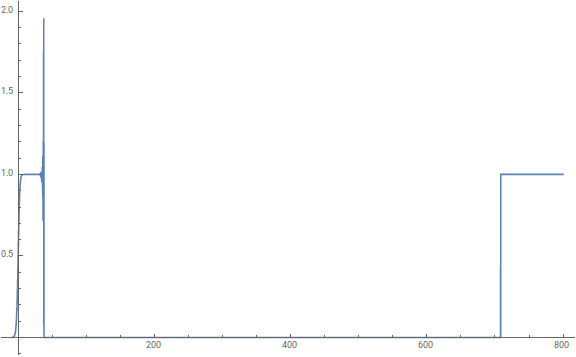
\includegraphics[width=0.49\textwidth]{wa2}}\hfill
\caption{Wykresy wykonane za pomocą programu \emph{Wolfram Alpha}} \label{fig:zad2-wa}
\end{figure}
\noindent Obliczona przez program granica $\mathop {\lim }\limits_{x \to \infty}$ funkcji \eqref{eq:zad2} wynosi $1$. Taki sam wynik został uzyskany przez rozwiązanie analityczne:
\begin{equation}
\begin{aligned}
\mathop {\lim }\limits_{x \to \infty} f(x) &= \mathop {\lim }\limits_{x \to \infty} e^x \ln(1 + e^{-x}) = \mathop {\lim }\limits_{x \to \infty} \dfrac{\ln(1 + e^{-x})}{e^{-x}} = \left[\dfrac{0}{0}\right] \stackrel{H}{=} \mathop {\lim }\limits_{x \to \infty} \dfrac{(\ln(1 + e^{-x}))'}{(e^{-x})'} = \\ 
&= \mathop {\lim }\limits_{x \to \infty} \dfrac{\frac{1}{1 + e^{-x}}\times -e^{-x}}{-e^{-x}} = \mathop {\lim }\limits_{x \to \infty} \dfrac{1}{1 + e^{-x}} = 1. \nonumber
\end{aligned}
\end{equation}

\subsection{Wnioski}

\section{Układ równań i wskaźnik uwarunkowania}

\subsection{Opis problemu}

Rozwiązanie układu równań liniowych $\mathbf{Ax} = \mathbf{b}$ dla danej macierzy współczynników $\mathbf{A} \in \mathbb{R}^{n\times n}$ i wektora prawych stron $\mathbf{b} \in \mathbb{R}^n$. \\
Macierz $\mathbf{A}$ zadana była w następujący sposób:
\begin{enumerate}[(a)]
\item \emph{macierz Hilberta} $\mathbf{H}_n$ stopnia $n$,
\item \emph{macierz losowa} $\mathbf{R}_n^c$ stopnia $n$ o danym wskaźniku uwarunkowania $c$.
\end{enumerate}
Wektor $\mathbf{b}$ natomiast jako $\mathbf{b} = \mathbf{Ax}$, gdzie $\mathbf{A}$ jest wygenerowaną macierzą, a $\mathbf{x} = (1, \dots, 1)^{T}$, tak aby było znane dokładne rozwiązanie dla $\mathbf{A}$ i $\mathbf{b}$. \\
Układ równań $\mathbf{Ax} = \mathbf{b}$ należało rozwiązać za pomocą dwóch algorytmów:
\begin{enumerate}[(i)]
\item \emph{metodą eliminacji Gaussa}: $\mathbf{x} = \mathbf{A} \backslash \mathbf{b}$,
\item \emph{metodą macierzy odwrotnej}: $\mathbf{x} = \mathbf{A}^{-1}\mathbf{b}$.
\end{enumerate}
Obliczone rozwiązania $\mathbf{\tilde{x}}$ dla różnych macierzy wejściowych należało porównać z rozwiązaniem dokładnym $\mathbf{x} = (1, \dots, 1)^{T}$ oraz obliczyć błędy względne. 


\subsection{Rozwiązanie}

Macierz Hilberta $\mathbf{H}_n$ z rosnącym stopniem $n > 1$ wygenerowano za pomocą funkcji $hilb(n)$, natomiast losową macierz $\mathbf{R}_n^c$, $n = 5,10,20$, z rosnącym wskaźnikiem uwarunkowania $c=1,10,10^3,10^7,10^{12},10^{16}$ stworzono przy użyciu funkcji $matcond(n, c)$. Dla każdej wygenerowanej macierzy rozwiązano układ równań metodą eliminacji Gaussa i macierzy odwrotnej, a także policzono błędy względne $\dfrac{||x - \tilde{x}||}{||x||}$ obu tych metod, wskaźniki uwarunkowania i rzędy macierzy.

\subsection{Wyniki}
Otrzymane wyniki dla macierzy Hilberta $\mathbf{H}_n$ prezentuje \Cref{table:2}, natomiast dla macierzy losowej $\mathbf{R}_n^c$ \Cref{table:3}, metoda eliminacji Gaussa jest oznaczona przez \texttt{GE}, a metoda macierzy odwrotnej przez \texttt{INV}.

\begin{table}[h]
        \centering
        \footnotesize
\begin{tabular}{|c|c
		|S[
        table-number-alignment = right,
		table-figures-integer  = 2,
		table-figures-decimal = 15,
		table-figures-exponent=3
		]
		|S[
        table-number-alignment = right,
		table-figures-integer  = 2,
		table-figures-decimal = 15,
		table-figures-exponent=3
		]
		|S[
        table-number-alignment = right,
		table-figures-integer  = 2,
		table-figures-decimal = 15,
		table-figures-exponent=3
		]|}
%\toprule
\hline
\multicolumn{5}{|c|}{Macierz Hilberta $\mathbf{H}_n$} \\ \hline
\multirow{2}{*}{Rozmiar} & \multirow{2}{*}{Rząd} & {\multirow{2}{*}{\texttt{COND}}} & \multicolumn{2}{c|}{Błędy względne} \\ \cline{4-5}
& & & {\texttt{GE}} & {\texttt{INV}} \\ \hline
1x1 & 1 & 1.0 & 0.0 & 0.0 \\
2x2 & 2 & 1.928147006790397e+01 & 5.661048867003676e-16 & 1.124015143811696e-15 \\
3x3 & 3 & 5.240567775860644e+02 & 8.022593772267726e-15 & 9.825526038180824e-15 \\
4x4 & 4 & 1.551373873892924e+04 & 4.451545960181209e-13 & 2.950477637286781e-13 \\
5x5 & 5 & 4.766072502425943e+05 & 1.682842629922719e-12 & 8.500055777753297e-12 \\
6x6 & 6 & 1.495105864225467e+07 & 2.618913302311624e-10 & 3.347413507036174e-10 \\
7x7 & 7 & 4.753673565831290e+08 & 1.260686722417155e-08 & 5.163959183577243e-09 \\
8x8 & 8 & 1.525757553806004e+10 & 1.026543065687064e-07 & 2.698715074276819e-07 \\
9x9 & 9 & 4.931537564468762e+11 & 4.832357120502150e-06 & 9.175846868614517e-06 \\
10x10 & 10 & 1.602441699254171e+13 & 6.329153722983848e-04 & 4.552142251740885e-04 \\
11x11 & 11 & 5.222677939280335e+14 & 1.154395859612211e-02 & 8.044466773431160e-03 \\
12x12 & 11 & 1.751473190709146e+16 & 2.975640310734787e-01 & 3.439293709120522e-01 \\
13x13 & 11 & 3.344143497338461e+18 & 2.375017867706776e+00 & 5.585796893150773e+00 \\
14x14 & 12 & 6.200786263161444e+17 & 5.281004646755168e+00 & 4.800641929017436e+00 \\
15x15 & 12 & 3.674392953467974e+17 & 1.177294734836712e+00 & 4.827357721257648e+00 \\
16x16 & 12 & 7.865467778431645e+17 & 2.056465582380410e+01 & 3.173646749626613e+01 \\
17x17 & 12 & 1.263684342666052e+18 & 1.774221463517907e+01 & 1.591033596260414e+01 \\
18x18 & 12 & 2.244630992918913e+18 & 4.276456441115942e+00 & 6.281223433472033e+00 \\
19x19 & 13 & 6.471953976541591e+18 & 2.211993729264891e+01 & 2.292561401563632e+01 \\
20x20 & 13 & 1.355365790868823e+18 & 1.493006966929400e+01 & 2.153949860251383e+01 \\
\hline

%\bottomrule
\end{tabular}
\caption{Wyniki obliczeń dla macierzy Hilberta $\mathbf{H}_n$}
\label{table:2}
\end{table}	

\begin{table}[h]
        \centering
        \footnotesize
\begin{tabular}{|c|c|l
		|S[
        table-number-alignment = right,
		table-figures-integer  = 2,
		table-figures-decimal = 15,
		table-figures-exponent=3
		]
		|S[
        table-number-alignment = right,
		table-figures-integer  = 2,
		table-figures-decimal = 15,
		table-figures-exponent=3
		]|}
%\toprule
\hline
\multicolumn{5}{|c|}{Macierz losowa $\mathbf{R}_n^c$} \\ \hline
\multirow{2}{*}{Rozmiar} & \multirow{2}{*}{Rząd} & {\multirow{2}{*}{\texttt{COND}}} & \multicolumn{2}{c|}{Błędy względne} \\ \cline{4-5}
& & & {\texttt{GE}} & {\texttt{INV}} \\ \hline
5x5 & 5 & 1 & 1.404333387430680e-16 & 1.790180836524724e-16 \\
5x5 & 5 & 10 & 0.0 & 9.930136612989092e-17 \\
5x5 & 5 & 1000 & 6.467561325518618e-15 & 6.138840652485208e-15 \\
5x5 & 5 & $10^7$ & 2.932858554206356e-10 & 2.541421917682778e-10 \\
5x5 & 5 & $10^{12}$ & 2.431174605159248e-05 & 2.445937707560239e-05 \\
5x5 & 4 & $10^{16}$ & 9.228482506511224e-02 & 1.358024596793109e-01 \\
10x10 & 10 & 1 & 2.328823463338184e-16 & 2.302207463925367e-16 \\
10x10 & 10 & 10 & 5.324442579404919e-16 & 5.916561726981507e-16 \\
10x10 & 10 & 1000 & 7.659734318226236e-16 & 1.167815308046354e-14 \\
10x10 & 10 & $10^7$ & 2.568414379855613e-10 & 2.258463845088549e-10 \\
10x10 & 10 & $10^{12}$ & 1.951994704671510e-05 & 2.174813032517800e-05 \\
10x10 & 9 & $10^{16}$ & 3.178399241163815e-01 & 3.516778693816187e-01 \\
20x20 & 20 & 1 & 5.495323605393213e-16 & 4.557326905135503e-16 \\
20x20 & 20 & 10 & 5.087681048627601e-16 & 4.071658748137585e-16 \\
20x20 & 20 & 1000 & 5.808917732317164e-15 & 3.747228857827342e-15 \\
20x20 & 20 & $10^7$ & 1.511216720479130e-10 & 1.241078754561024e-10 \\
20x20 & 20 & $10^{12}$ & 4.740084259557948e-05 & 4.819264617327459e-05 \\
20x20 & 19 & $10^{16}$ & 8.613420159130484e-01 & 8.466277602660599e-01 \\
\hline

%\bottomrule
\end{tabular}
\caption{Wyniki obliczeń dla macierzy losowej $\mathbf{R}_n^c$}
\label{table:3}
\end{table}	

\subsection{Wnioski}

\section{,,Złośliwy wielomian'' Wilkinsona}

\subsection{Opis problemu}

Obliczenie dwudziestu zer wielomianu Wilkinsona $p$, tj. $p(x) = (x-20)(x-19)\dots(x-2)(x-1)$ w postaci naturalnej $P$ i sprawdzenie otrzymanych pierwiastków $z_k$ poprzez obliczenie $|P(z_k)|$, $|p(z_k)|$ i $|z_k-k|$ dla $1\leq x\leq 20$. Powtórzenie eksperymentu Wilkinsona, tj. zmiana współczynnika $-210$ przy $x^{19}$ na $-210-2^{-23}$ i wyjaśnienie zaistniałego zjawiska.

\subsection{Rozwiązanie}

Do rozwiązania zadania użyto pakietu \texttt{Polynomials}. Miejsca zerowe wielomianu $P$ utworzonego z danych współczynników za pomocą funkcji \texttt{Poly} obliczono przy użyciu funkcji \texttt{roots}. Za pomocą funkcji \texttt{poly} stworzono natomiast wielomian $p$. Funkcja \texttt{polyval} posłużyła do obliczenia wartości wielomianów $P$ i $p$ w zadanych punktach. Obliczony został również błąd bezwzględny obliczonych pierwiastków wielomianu $P$. Podobne operacje zostały wykonane dla wielomianu $P$ z zaburzonym współczynnikiem przy $x^{19}$.

\subsection{Wyniki}

\Cref{table:4} przedstawia obliczone pierwiastki wielomianu $P$ oraz $|P(z_k)|$, $|p(z_k)|$ i $|z_k-k|$, natomiast \Cref{table:5} prezentuje te wartości dla wielomianu $P$ z zaburzonym współczynnikiem.

\begin{table}[h]
        \centering
        \footnotesize
\begin{tabular}{c
		|S[
        table-number-alignment = right,
		table-figures-integer  = 1,
		table-figures-decimal = 12,
		table-figures-exponent=2
		]
		|S[
        table-number-alignment = right,
		table-figures-integer  = 1,
		table-figures-decimal = 12,
		table-figures-exponent=2
		]
		|S[
        table-number-alignment = right,
		table-figures-integer  = 1,
		table-figures-decimal = 12,
		table-figures-exponent=2
		]}
%\toprule
{$k$} & {$|P(z_k)|$} & {$|p(z_k)|$} & {$|z_k-k|$} \\ \hline
1 & 2.746295274547e+13 & 2.746278890701e+13 & 1.907087633626e-04 \\
2 & 1.027837616282e+13 & 1.027823565670e+13 & 1.909818299438e-03 \\
3 & 7.199554861056e+12 & 7.199447475200e+12 & 9.078647283520e-03 \\
4 & 3.777623778304e+12 & 3.777532946944e+12 & 2.542714623741e-02 \\
5 & 1.555027751936e+12 & 1.554961097216e+12 & 5.371328339203e-02 \\
6 & 6.139877534720e+11 & 6.139384156160e+11 & 7.549379969948e-02 \\
7 & 3.653832509440e+11 & 3.653447936000e+11 & 8.524440819787e-02 \\
8 & 2.157236290560e+11 & 2.156963307520e+11 & 7.431403244734e-02 \\
9 & 7.216771584000e+10 & 7.214665062400e+10 & 4.671674615314e-02 \\
10 & 3.575989555200e+10 & 3.574346905600e+10 & 2.502293290932e-02 \\
11 & 1.270712678400e+10 & 1.269690726400e+10 & 9.586957518275e-03 \\
12 & 4.465326592000e+09 & 4.457859584000e+09 & 2.915294362053e-03 \\
13 & 1.682691072000e+09 & 1.678497280000e+09 & 6.441703922384e-04 \\
14 & 4.803983360000e+08 & 4.782909440000e+08 & 1.020027930076e-04 \\
15 & 1.201520640000e+08 & 1.188249600000e+08 & 1.075417522678e-05 \\
16 & 2.411468800000e+07 & 2.334668800000e+07 & 6.657697912971e-07 \\
17 & 3.106816000000e+06 & 2.844672000000e+06 & 1.626246826092e-08 \\
18 & 2.094080000000e+05 & 3.015680000000e+05 & 4.079034887638e-10 \\
19 & 1.817600000000e+05 & 1.981440000000e+05 & 2.831823664451e-11 \\
20 & 3.635200000000e+04 & 3.840000000000e+04 & 3.010924842783e-13 \\
%\bottomrule
\end{tabular}
\caption{Obliczone wartości dla wielomianu $P$}
\label{table:4}
\end{table}

\begin{table}[h]
        \centering
        \scriptsize
\begin{tabular}{c|c
		|S[
        table-number-alignment = right,
		table-figures-integer  = 1,
		table-figures-decimal = 12,
		table-figures-exponent=1
		]
		|S[
        table-number-alignment = right,
		table-figures-integer  = 1,
		table-figures-decimal = 12,
		table-figures-exponent=1
		]
		|S[
        table-number-alignment = right,
		table-figures-integer  = 1,
		table-figures-decimal = 12,
		table-figures-exponent=1
		]}
%\toprule
{$k$} & {$z_k$} & {$|P(z_k)|$} & {$|p(z_k)|$} & {$|z_k-k|$} \\ \hline
1&20.846910215194789&1.114453504512e+13&1.374373319725e+18&8.469102151948e-01 \\
2&19.502442368818102 + 1.940331978642903i&9.539424609818e+12&4.252502487993e+17&2.004329444310e+00 \\
3&19.502442368818102 - 1.940331978642903i&9.539424609818e+12&4.252502487993e+17&2.454021446313e+00 \\
4&16.730744879792670 + 2.812624896721978i&3.315103475982e+11&2.742089401676e+16&2.825483521350e+00 \\
5&16.730744879792670 - 2.812624896721978i&3.315103475982e+11&2.742089401676e+16&2.906001873538e+00 \\
6&13.992406684487216 + 2.518824425710844i&1.061206453308e+11&9.545941595184e+14&2.712880531285e+00 \\
7&13.992406684487216 - 2.518824425710844i&1.061206453308e+11&9.545941595184e+14&2.518835871191e+00 \\
8&11.793890586174369 + 1.652477136407579i&3.357756113172e+10&3.296021414130e+13&2.045820276678e+00 \\
9&11.793890586174369 - 1.652477136407579i&3.357756113172e+10&3.296021414130e+13&1.665281290598e+00 \\
10&10.095455630535774 + 0.644932823624069i&7.143113638036e+09&1.491263381675e+12&1.110918027272e+00 \\
11&10.095455630535774 - 0.644932823624069i&7.143113638036e+09&1.491263381675e+12&6.519586830380e-01 \\
12&8.915816367932559&3.065575424000e+09&1.371743170560e+11&8.418363206744e-02 \\
13&8.007772029099446&1.072547328000e+09&1.852548659200e+10&7.772029099446e-03 \\
14&6.999602070422420&3.881231360000e+08&1.757670912000e+09&3.979295775798e-04 \\
15&6.000020476673031&1.291484160000e+08&2.061204480000e+08&2.047667303096e-05 \\
16&4.999998573887910&3.946393600000e+07&4.330393600000e+07&1.426112089753e-06 \\
17&4.000000089724362&1.046784000000e+07&1.072998400000e+07&8.972436216226e-08 \\
18&2.999999996603420&2.221568000000e+06&2.295296000000e+06&3.396579906223e-09 \\
19&2.000000000055037&3.491840000000e+05&3.655680000000e+05&5.503730804435e-11 \\
20&0.999999999999836&2.099200000000e+04&2.201600000000e+04&1.643130076445e-13 \\
%\bottomrule
\end{tabular}
\caption{Obliczone wartości dla wielomianu $P$ z zaburzonym współczynnikiem przy $x^{19}$}
\label{table:5}
\end{table}

\subsection{Wnioski}

\section{Model wzrostu populacji}

\subsection{Opis problemu}

Zbadanie modelu wzrostu populacji (model logistyczny)
\begin{align}
p_{n+1} := p_n + rp_n(1-p_n), \ \textrm{dla} \ n = 0, 1, \dots,
\label{eq:zad5}
\end{align}
gdzie $r$ jest pewną daną stałą, $r(1-p_n)$ jest czynnikiem wzrostu populacji, a $p_0$ jest wielkością populacji stanowiącą procent maksymalnej wielkości populacji dla danego stanu środowiska. \\
\newline
W tym celu należało przeprowadzić następujące eksperymenty.
\begin{enumerate}[(i)]
\item Wykonanie 40 iteracji wyrażenia \eqref{eq:zad5} w arytmetyce \texttt{Float32} dla danych $p_0 = 0.01$ i $r = 3$. Ponowne wykonanie 40 iteracji wyrażenia \eqref{eq:zad5} z niewielką modyfikacją tj. wykonanie 10 iteracji, zatrzymanie, zastosowanie obcięcia wyniku odrzucając cyfry po trzecim miejscu po przecinku (daje to liczbę $0.722$) i kontynuowanie dalej obliczenia (do 40-stej iteracji) tak, jak gdyby był to ostatni wynik na wyjściu. Porównanie wyników obu iteracji.
\item Wykonanie 40 iteracji wyrażenia \eqref{eq:zad5} dla danych $p_0 = 0.01$ i $r = 3$ w arytmetyce \texttt{Float32} i \texttt{Float64}. Porównanie wyników iteracji dla obu arytmetyk.
\end{enumerate}

\subsection{Rozwiązanie}

Zaimplementowano podany model wzrostu populacji i za pomocą stworzonej funkcji obliczono wyniki dla odpowiedniej liczby iteracji.

\subsection{Wyniki}

Zestawienie wyników dla obu eksperymentów prezentują odpowiednio \Cref{table:6} oraz \Cref{table:7}.

\begin{table}[h]
        \centering
        \footnotesize
\begin{tabular}{c
		|S[
        table-number-alignment = right,
		table-figures-integer  = 2,
		table-figures-decimal = 10,
		%table-figures-exponent=6
		]
		|S[
        table-number-alignment = right,
		table-figures-integer  = 2,
		table-figures-decimal = 10,
		%table-figures-exponent=6
		]}
%\toprule
Iteracja & {Bez modyfikacji} & {Z modyfikacją} \\ \hline
1&0.0397&0.0397 \\
2&0.15407173&0.15407173 \\
3&0.5450726&0.5450726 \\
4&1.2889781&1.2889781 \\
5&0.1715188&0.1715188 \\
10&0.7229306&0.722 \\
11&1.3238364&1.3241479 \\
12&0.037716985&0.036488414 \\
15&1.2704837&1.2572169 \\
17&0.7860428&0.9010855 \\
19&0.16552472&0.577893 \\
20&0.5799036&1.3096911 \\
25&1.0070806&1.0929108 \\
30&0.7529209&1.3191822 \\
35&1.021099&0.034241438 \\
40&0.25860548&1.093568 \\
%\bottomrule
\end{tabular}
\caption{Wybrane wyniki kolejnych iteracji modelu logistycznego w arytmetyce \texttt{Float32} bez modyfikacji i z obcięciem wyniku 10 iteracji od 3 miejsca po przecinku}
\label{table:6}
\end{table}	

\begin{table}[h]
        \centering
        \footnotesize
\begin{tabular}{c
		|S[
        table-number-alignment = right,
		table-figures-integer  = 2,
		table-figures-decimal = 10,
		%table-figures-exponent=6
		]
		|S[
        table-number-alignment = right,
		table-figures-integer  = 2,
		table-figures-decimal = 18,
		%table-figures-exponent=6
		]}
%\toprule
Iteracja & {Float32} & {Float64} \\ \hline
1&0.0397&0.0397 \\
2&0.15407173&0.15407173000000002 \\
3&0.5450726&0.5450726260444213 \\
4&1.2889781&1.2889780011888006 \\
5&0.1715188&0.17151914210917552 \\
10&0.7229306&0.722914301179573 \\
15&1.2704837&1.2702617739350768 \\
20&0.5799036&0.5965293124946907 \\
25&1.0070806&1.315588346001072 \\
26&0.9856885&0.07003529560277899 \\
27&1.0280086&0.26542635452061003 \\
30&0.7529209&0.37414648963928676 \\
35&1.021099&0.9253821285571046 \\
39&1.2652004&0.0029091569028512065 \\
40&0.25860548&0.011611238029748606 \\
%\bottomrule
\end{tabular}
\caption{Wybrane wyniki kolejnych iteracji modelu logistycznego w arytmetyce \texttt{Float32} i \texttt{Float64}}
\label{table:7}
\end{table}

\noindent Dla lepszego ukazania rozbieżności pomiędzy kolejnymi iteracjami w eksperymentach zostały narysowane wykresy (\Cref{fig:zad5}) przedstawiające wartość bezwzględną różnic otrzymanych wyników.

\begin{figure}[h]
\centering
\subfloat[\texttt{Float32} bez modyfikacji i z obcięciem \label{fig:zad5-1}]{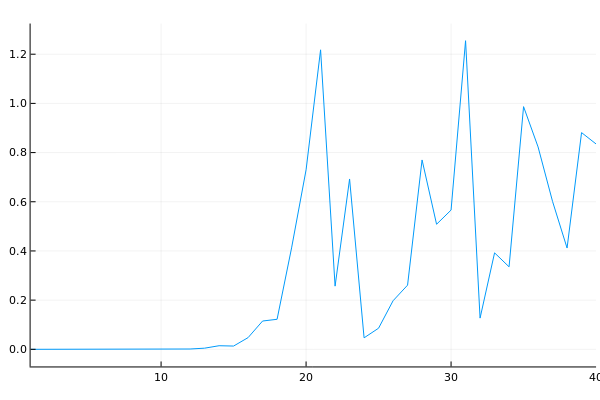
\includegraphics[width=0.49\textwidth]{zad5(1)}}\hfill
\subfloat[\texttt{Float32} i \texttt{Float64} \label{fig:zad5-2}] {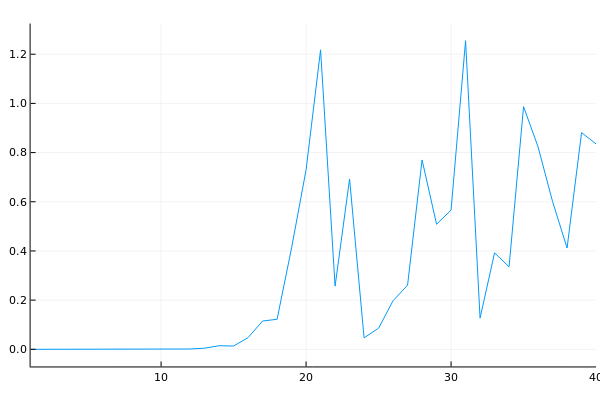
\includegraphics[width=0.49\textwidth]{zad5(2)}}\hfill
\caption{Wykresy przedstawiają różnicę pomiędzy kolejnymi wynikami iteracji} \label{fig:zad5}
\end{figure}

\subsection{Wnioski}

\section{Iterowanie funkcji kwadratowej}

\subsection{Opis problemu}

Zbadanie zachowania równania rekurencyjnego
\begin{align}
x_{n+1} := x^2_n + c, \ \textrm{dla} \ n = 0,1,\dots,
\label{eq:zad6}
\end{align}
gdzie $c$ jest pewną daną stałą, dla następujących danych:
\begin{enumerate}[(i)]
\item $c = -2$ i $x_0 = 1$
\item $c = -2$ i $x_0 = 2$
\item $c = -2$ i $x_0 = 1.99999999999999$
\item $c = -1$ i $x_0 = 1$
\item $c = -1$ i $x_0 = -1$
\item $c = -1$ i $x_0 = 0.75$
\item $c = -1$ i $x_0 = 0.25$
\end{enumerate}
W tym celu należało wykonać 40 iteracji wyrażenia \eqref{eq:zad6} i zaobserwować zachowanie generowanych ciągów, a także przeprowadzić iterację graficzną \eqref{eq:zad6}. 

\subsection{Rozwiązanie}

\subsection{Wyniki}

\begin{table}[h]
        \centering
        \scriptsize
\begin{tabular}{c
		|S[
        table-number-alignment = right,
		table-figures-integer  = 2,
		table-figures-decimal = 1,
		%table-figures-exponent=6
		]
		|S[
        table-number-alignment = right,
		table-figures-integer  = 2,
		table-figures-decimal = 1,
		%table-figures-exponent=6
		]
		|S[
        table-number-alignment = right,
		table-figures-integer  = 2,
		table-figures-decimal = 16,
		%table-figures-exponent=6
		]
		|S[
        table-number-alignment = right,
		table-figures-integer  = 2,
		table-figures-decimal = 1,
		%table-figures-exponent=6
		]
		|S[
        table-number-alignment = right,
		table-figures-integer  = 2,
		table-figures-decimal = 1,
		%table-figures-exponent=6
		]
		|S[
        table-number-alignment = right,
		table-figures-integer  = 2,
		table-figures-decimal = 16,
		table-figures-exponent=2
		]
		|S[
        table-number-alignment = right,
		table-figures-integer  = 2,
		table-figures-decimal = 15,
		table-figures-exponent=2
		]}
%\toprule
\multirow{2}{*}{It.} & \multicolumn{3}{c|}{$c=-2$} & \multicolumn{4}{c}{$c=-1$}  \\ \cline{2-8}
&{$x_0$=1}&{$x_0$=2}&{$x_0$=1.99999999999999}&{$x_0$=1}&{$x_0$=-1}&{$x_0$=0.75}&{$x_0$=0.25} \\ \hline
1&-1.0&2.0&1.99999999999996&0.0&0.0&-0.4375&-0.9375 \\
2&-1.0&2.0&1.9999999999998401&-1.0&-1.0&-0.80859375&-0.12109375 \\
3&-1.0&2.0&1.9999999999993605&0.0&0.0&-0.3461761474609375&-0.9853363037109375 \\
4&-1.0&2.0&1.999999999997442&-1.0&-1.0&-0.8801620749291033&-0.029112368589267135 \\
5&-1.0&2.0&1.9999999999897682&0.0&0.0&-0.2253147218564956&-0.9991524699951226 \\
6&-1.0&2.0&1.9999999999590727&-1.0&-1.0&-0.9492332761147301&-0.0016943417026455965 \\
7&-1.0&2.0&1.999999999836291&0.0&0.0&-0.0989561875164966&-0.9999971292061947 \\
8&-1.0&2.0&1.9999999993451638&-1.0&-1.0&-0.9902076729521999&-5.741579369278327e-6 \\
9&-1.0&2.0&1.9999999973806553&0.0&0.0&-0.01948876442658909&-0.9999999999670343 \\
10&-1.0&2.0&1.999999989522621&-1.0&-1.0&-0.999620188061125&-6.593148249578462e-11 \\
11&-1.0&2.0&1.9999999580904841&0.0&0.0&-0.0007594796206411569&-1.0 \\
12&-1.0&2.0&1.9999998323619383&-1.0&-1.0&-0.9999994231907058&0.0 \\
13&-1.0&2.0&1.9999993294477814&0.0&0.0&-1.1536182557003727e-6&-1.0 \\
14&-1.0&2.0&1.9999973177915749&-1.0&-1.0&-0.9999999999986692&0.0 \\
15&-1.0&2.0&1.9999892711734937&0.0&0.0&-2.6616486792363503e-12&-1.0 \\
16&-1.0&2.0&1.9999570848090826&-1.0&-1.0&-1.0&0.0 \\
17&-1.0&2.0&1.999828341078044&0.0&0.0&0.0&-1.0 \\
18&-1.0&2.0&1.9993133937789613&-1.0&-1.0&-1.0&0.0 \\
19&-1.0&2.0&1.9972540465439481&0.0&0.0&0.0&-1.0 \\
20&-1.0&2.0&1.9890237264361752&-1.0&-1.0&-1.0&0.0 \\
21&-1.0&2.0&1.9562153843260486&0.0&0.0&0.0&-1.0 \\
22&-1.0&2.0&1.82677862987391&-1.0&-1.0&-1.0&0.0 \\
23&-1.0&2.0&1.3371201625639997&0.0&0.0&0.0&-1.0 \\
24&-1.0&2.0&-0.21210967086482313&-1.0&-1.0&-1.0&0.0 \\
25&-1.0&2.0&-1.9550094875256163&0.0&0.0&0.0&-1.0 \\
26&-1.0&2.0&1.822062096315173&-1.0&-1.0&-1.0&0.0 \\
27&-1.0&2.0&1.319910282828443&0.0&0.0&0.0&-1.0 \\
28&-1.0&2.0&-0.2578368452837396&-1.0&-1.0&-1.0&0.0 \\
29&-1.0&2.0&-1.9335201612141288&0.0&0.0&0.0&-1.0 \\
30&-1.0&2.0&1.7385002138215109&-1.0&-1.0&-1.0&0.0 \\
31&-1.0&2.0&1.0223829934574389&0.0&0.0&0.0&-1.0 \\
32&-1.0&2.0&-0.9547330146890065&-1.0&-1.0&-1.0&0.0 \\
33&-1.0&2.0&-1.0884848706628412&0.0&0.0&0.0&-1.0 \\
34&-1.0&2.0&-0.8152006863380978&-1.0&-1.0&-1.0&0.0 \\
35&-1.0&2.0&-1.3354478409938944&0.0&0.0&0.0&-1.0 \\
36&-1.0&2.0&-0.21657906398474625&-1.0&-1.0&-1.0&0.0 \\
37&-1.0&2.0&-1.953093509043491&0.0&0.0&0.0&-1.0 \\
38&-1.0&2.0&1.8145742550678174&-1.0&-1.0&-1.0&0.0 \\
39&-1.0&2.0&1.2926797271549244&0.0&0.0&0.0&-1.0 \\
40&-1.0&2.0&-0.3289791230026702&-1.0&-1.0&-1.0&0.0 \\
%\bottomrule
\end{tabular}
\caption{Wybrane wyniki kolejnych iteracji modelu logistycznego w arytmetyce \texttt{Float32} i \texttt{Float64}}
\label{table:8}
\end{table}

\subsection{Wnioski}


%\begin{algorithm}[h]
%\caption{Wyznaczanie epsilonów maszynowych.}
%\label{alg:macheps}
%\SetKwData{Macheps}{macheps}\SetKwData{NMacheps}{new\_{}macheps}
%
%\Macheps $\leftarrow 1.0$\;
%\NMacheps $\leftarrow 1.0$\;
%\While {$1.0 + \NMacheps > 1.0$}{
%$\Macheps\leftarrow \NMacheps$\;
%$\NMacheps \leftarrow \NMacheps / 2.0$\;
%}
%\Return \Macheps
%\end{algorithm}

\end{document}
